\section{Developing the New Oracles}
\label{sec:developing-oracles}
To evaluate method-tracking tools, it is essential to have reliable ground truths against which the correctness of the tools can be measured. An oracle created in a purely manual manner remains vulnerable to internal validity threats due to its substantial dependence on human judgment. Manual efforts are prone to inconsistencies, oversight, and bias, particularly when dealing with complex software evolution patterns. Constructing such an oracle is also highly impractical for large-scale real-world codebases, which often consist of thousands of files and methods. During software evolution, methods may undergo renaming, move across files, or be refactored in tandem with other code changes, including modifications to their signatures and bodies. These transformations may occur within a single commit or span across multiple commits, making manual tracking extremely error-prone and difficult to scale.

Therefore, a hybrid approach was adopted that combined automated analysis with human verification. Method histories were collected with multiple state-of-the-art tools, each with distinct strengths and weaknesses, and each reported change was manually validated to ensure high precision and recall. This union-based strategy was inspired by an observation in the original \textit{CodeShovel} research: although \textit{CodeShovel} outperformed all other tools, it occasionally missed method change commits that were correctly identified by those other tools.

To find potential change commits that were not captured by any of the tools, the first two authors used the \texttt{git log} command to trace changed files (not methods) containing the methods of interest, manually verifying whether any were actual change commits.
These two authors have 8+ years of industry experience in software development and \texttt{Git-based} project management. This process uncovered 43 additional commits. While this quick manual process may not reveal all missing commits, finding only 43 out of 9,005 total suggests that the union set already had high recall.

Each method’s history was then independently reviewed by these two authors. Inter-rater agreement was evaluated using Cohen’s Kappa~\cite{cohen_coefficient_1960}, which yielded a value of 0.97, indicating an almost perfect~\cite{viera2005understanding} level of agreement between the two authors. Out of 9,005 commits in the union set, only 66 had disagreements, which arose from: (i) introduction of new overloaded versions with the same name, and (ii) different tools identifying different methods due to varying body-similarity thresholds. These disagreements were resolved through Zoom discussions by examining function call locations and contextual information in the Java file.
Figure~\ref{fig:oracle-construction-process} summarizes the oracle construction process. The next sections describe the two oracles developed here.

\begin{figure}[t]
\centering
% \resizebox{\columnwidth}{!}{%
% \input{figure/method-history-refinement-process}
% } % end resizebox
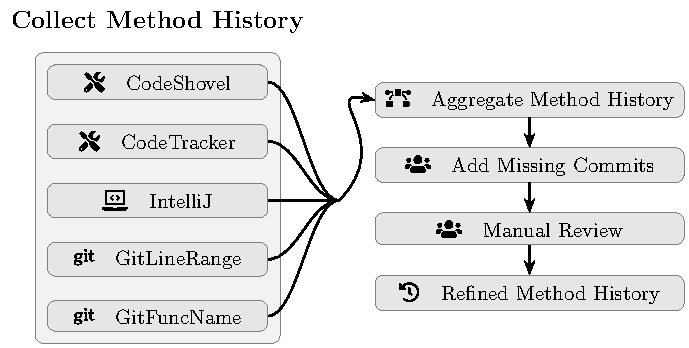
\includegraphics[width=\textwidth]{figure/method-history-refinement-process.pdf}
\caption{The process used to generate accurate oracles. The union of the change commits reported by all tools was first created, missing commits were added, and false positives were then removed.}
% \Description{The process to generate accurate oracles. We first took the union of the change commits reported by all tools, added missing commits, and then removed the false positives.}
\label{fig:oracle-construction-process}
\end{figure}

\subsection{Updating the CodeShovel Oracle}
\label{sec:updating-codeshovel-oracle}
Using the five tools (\textit{CodeShovel}, \textit{CodeTracker}, \textit{IntelliJ}, \textit{GitLineRange}, and \textit{GitFuncName}), method change histories were collected for the 200 methods used in the original \textit{CodeShovel} study. For \textit{CodeShovel} and \textit{CodeTracker}, the tools were used as library dependencies, as they are publicly available on \texttt{GitHub}. For \textit{IntelliJ}, each project was manually imported, the specific commits were checked out, the target files and methods were located, and the \texttt{Show History for Selection} option was used to generate the method change histories. For the Git-based tools, shell commands namely \texttt{git log <commit> --no-merges -L :<funcname>:<file>} and \texttt{git log <commit> --no-merges \allowbreak{}-L <start>,<end>:<file>} were executed to collect method histories. Finally, the method change histories from all five tools were aggregated into a unified commit history, producing a union of the commit histories of all tools. The missing commits mentioned earlier were also added. The commit histories were then sorted in reverse chronological order by their commit timestamp. Next, each method change commit was manually inspected to verify its logical validity by comparing it with its parent commit. This process is repeated iteratively for each subsequent commit until all commits have been thoroughly examined. At the end of this process, a complete and accurate method history oracle was obtained for the 200 methods. These 200 methods are referred to as the corrected \textit{CodeShovel} oracle.

\subsection{Constructing the HistoryFinder Oracle}
\label{sec:history-finder-oracle}
The \textit{HistoryFinder} oracle was created from 20 additional open-source Java projects selected from \texttt{GitHub}. To ensure high-quality projects~\cite{kalliamvakou_promises_2014}, popular projects were selected based on a high number of stars and forks. Each project was also required to have at least 2,000 commits so that enough method change commits could be found for the selected methods from these projects.
Table \ref{tab:history-finder-repository-list} presents the list of selected projects along with their number of commits, Java files, methods, and their respective star and fork counts. From each project, 10 methods were randomly selected, recording their file names, method names, and start and end line numbers, resulting in a total of 200 methods. The same approach described in section \ref{sec:updating-codeshovel-oracle} was then followed to generate the change history oracle for this new set of 200 methods.

\begin{table}[ht]
\centering
\caption{Overview of the 20 Java repositories used for the \textit{HistoryFinder} oracle, including commit counts, source files, methods, and popularity metrics (stars and forks).}
\label{tab:history-finder-repository-list}
\resizebox{\linewidth}{!}{%
\begin{tabular}{lrrrrr}
\toprule
\textbf{Repository} & \textbf{\# Commits} & \textbf{\# Files} & \textbf{\# Methods} & \textbf{\# Stars} & \textbf{\# Forks} \\
\midrule
    auto & 2,570 & 317 & 4,211 & 10,441 & 1,202 \\
    cassandra & 31,705 & 4,926 & 76,475 & 8,913 & 3,641 \\
    dagger & 5,592 & 1,436 & 8,043 & 17,467 & 2,019 \\
    dubbo & 9,428 & 3,713 & 28,365 & 40,581 & 26,442 \\
    fastjson & 7,216 & 2,997 & 19,239 & 25,761 & 6,498 \\
    glide & 3,395 & 724 & 8,804 & 34,718 & 6,128 \\
    guice & 2,444 & 615 & 6,981 & 12,521 & 1,673 \\
    Hystrix & 2,354 & 415 & 6,436 & 24,160 & 4,708 \\
    j2objc & 6,314 & 5,119 & 106,062 & 5,998 & 972 \\
    jenkins & 37,342 & 1,779 & 21,660 & 23,363 & 8,834 \\
    jmeter & 32,202 & 1,526 & 16,138 & 8,468 & 2,116 \\
    kafka & 20,356 & 4,632 & 62,991 & 29,077 & 14,030 \\
    MPAndroidChart & 2,074 & 223 & 2,447 & 37,694 & 9,027 \\
    netty & 19,625 & 1,973 & 22,902 & 33,578 & 15,974 \\
    pulsar & 20,639 & 4,153 & 44,183 & 14,323 & 3,601 \\
    rocketmq & 8,918 & 1,581 & 17,155 & 21,361 & 11,727 \\
    RxJava & 7,698 & 1,884 & 33,994 & 47,951 & 7,602 \\
    shardingsphere & 43,769 & 7,765 & 34,921 & 20,035 & 6,775 \\
    tomcat & 77,289 & 2,705 & 42,021 & 7,619 & 5,062 \\
    zxing & 3,816 & 499 & 3,293 & 32,923 & 9,365 \\
\bottomrule
\end{tabular}
}
\end{table}
